\documentclass[aspectratio=43]{beamer}

\usepackage[T2A]{fontenc}
\usepackage[utf8]{inputenc}
\usepackage[english,russian]{babel}
\usepackage{amsmath,amssymb,amsbsy}
\usepackage{graphicx}
\usepackage{booktabs}
\usepackage{microtype}
\usefonttheme[onlymath]{serif}

%% ====================================================================
%%  Тема в стиле защит ФПМИ: красный заголовок в серой рамке,
%%  синие подзаголовки и структура внутри слайда.
%% ====================================================================
\usetheme{default}
\useinnertheme{default}
\useoutertheme{default}
\setbeamertemplate{navigation symbols}{}

\definecolor{titlered}{RGB}{176,42,42}     % красный — заголовки кадров
\definecolor{slideblue}{RGB}{45,55,140}    % синий — структура и подзаголовки
\definecolor{titlebar}{RGB}{236,236,238}   % светло-серая рамка заголовка

%% синий — вся «структура» (маркеры, блоки, акценты)
\setbeamercolor{structure}{fg=slideblue}
\setbeamercolor{title}{fg=titlered}
\setbeamercolor{item}{fg=slideblue}
\setbeamercolor{block title}{fg=slideblue}

%% красный заголовок кадра на серой плашке во всю ширину
\setbeamercolor{frametitle}{fg=titlered,bg=titlebar}
\setbeamerfont{frametitle}{series=\bfseries}
\setbeamerfont{title}{series=\bfseries}

%% собственная боковая граница (без внутренних макросов beamer с @)
\newlength{\fpmargin}\setlength{\fpmargin}{0.8cm}
\setbeamersize{text margin left=\fpmargin,text margin right=\fpmargin}

%% отступ текста заголовка кадра от левого края плашки (больше поля текста,
%% чтобы заголовок не липнул к краю страницы)
\newlength{\fptitleindent}\setlength{\fptitleindent}{1.4cm}

\setbeamertemplate{frametitle}{%
  \nointerlineskip%
  \hspace*{-\fpmargin}%
  \begin{beamercolorbox}[wd=\paperwidth,sep=0pt,%
      leftskip=\fptitleindent,rightskip=\fpmargin]{frametitle}%
    \vskip0.32cm\usebeamerfont{frametitle}\insertframetitle\vskip0.32cm%
  \end{beamercolorbox}%
  \vskip0.4em%
}

%% Нижний колонтитул: номер слайда справа
\setbeamertemplate{footline}{%
  \hfill\usebeamerfont{page number in head/foot}%
  \color{slideblue!70}\scriptsize\insertframenumber\,/\,\inserttotalframenumber\hspace*{1.5em}\vskip4pt%
}

%% Маркеры списков
\setbeamertemplate{itemize item}{\color{slideblue}\textbullet}
\setbeamertemplate{itemize subitem}{\color{slideblue!70}--}
\setbeamertemplate{enumerate item}{\color{slideblue}\insertenumlabel.}

%% Синий подзаголовок-блок внутри слайда («Проблема», «Цель», ...)
\newcommand{\heading}[1]{\smallskip{\color{slideblue}\bfseries #1}\par\nobreak\smallskip}
%% Компактная ссылка на источник
\newcommand{\cit}[1]{{\footnotesize\color{slideblue!75}[#1]}}

\title{Применение методов каузального вывода при анализе зависимостей между оптимизирующими проходами LLVM-компилятора}

\begin{document}

%% ================= Слайд 1: титул =================
\begin{frame}[plain]
  \vfill
  \begin{center}
    \begin{beamercolorbox}[wd=0.92\paperwidth,sep=0.5cm,center,rounded=true]{frametitle}
      \usebeamerfont{title}\large
      Применение методов каузального вывода при анализе
      зависимостей между оптимизирующими проходами
      LLVM-компилятора
    \end{beamercolorbox}

    \vskip1.4em
    Белонин Владимир Викторович\\[0.3em]
    {\small группа М05-002д}\\[0.8em]
    {\small Научный руководитель:\\
      д-р техн. наук, проф. С.\,К.~Дулин\par}
    {\small Научный консультант:\\
      к.ф.-м.н., доцент Н.\,Н.~Ефанов\par}
    \vskip1.2em
    {\footnotesize
      Московский физико-технический институт (НИУ)\\
      Физтех-школа прикладной математики и информатики\\
      Кафедра интеллектуальных систем ФИЦ ИУ РАН\par}
    \vskip1.0em
    {\small Долгопрудный, 2026}
  \end{center}
  \vfill
\end{frame}

%% ================= Слайд 2: задача и актуальность =================
\begin{frame}{Порядок оптимизирующих проходов: задача и актуальность}
  \small
  \heading{Область}
  Оптимизирующий компилятор применяет десятки проходов; результат зависит не
  только от \emph{выбора} проходов, но и от \textbf{порядка} их применения~---
  это \emph{задача упорядочивания} (phase ordering).

  \heading{Масштаб и востребованность}
  \begin{itemize}
    \item В LLVM более 150 проходов; уже для 33~проходов
      (длина \texttt{-Oz}) число порядков проходов превышает $10^{49}$ \cit{Ashouri, 2018}.
    \item Специализированный порядок заметно улучшает метрику относительно
      \texttt{-O3}/\texttt{-Oz} \cit{Ashouri, 2018}.
  \end{itemize}
\end{frame}

%% ================= Слайд 3: ПОСТАНОВКА ЗАДАЧИ =================
\begin{frame}{Постановка задачи}
  \small
  \heading{Цель работы}
  Выявить \textbf{каузальные} зависимости между оптимизирующими проходами LLVM и
  построить интерпретируемые графы их взаимодействий~--- с отделением
  причинно-следственных связей от корреляционных.

  \heading{Задачи}
  \begin{enumerate}\setlength{\itemsep}{0pt}
    \item Сформулировать влияние порядка пары проходов как каузальный вопрос в
      модели потенциальных исходов.
    \item Спроектировать и провести рандомизированный эксперимент над порядком
      проходов.
    \item Оценить каузальные эффекты всех пар проходов с контролем множественной
      проверки гипотез.
    \item Построить каузальные графы на нескольких уровнях агрегации.
    \item Сравнить каузальный граф с корреляционным и оценить долю ложных связей.
    \item Исследовать гетерогенность эффектов порядка по типам программ.
  \end{enumerate}
\end{frame}

%% ================= Слайд 4: ПРОБЕЛ — корреляция не каузация =================
\begin{frame}{Существующие подходы и их ограничение}
  \heading{Три семейства методов}
  \begin{itemize}
    \item \textbf{Итеративная компиляция} \cit{Fursin, 2011}~--- перебор; дорого,
      результат не переносится между программами.
    \item \textbf{ML-предсказание порядка} \cit{Trofin, 2021; Cummins, 2022}~---
      «чёрный ящик»: не объясняет, \emph{почему} порядок лучше.
    \item \textbf{Корреляционные биграммы} \cit{Fursin, 2011}~--- связывают пары
      проходов с выигрышем по совместной встречаемости.
  \end{itemize}

  \begin{block}{Общий недостаток}
    \centering
    Ни один метод не отделяет \textbf{причину} от \textbf{корреляции}.\\
    То, что пара проходов часто встречается в выигрышных прогонах, не значит,
    что её порядок \emph{вызывает} выигрыш.
  \end{block}

  \heading{Каузальный вопрос работы}
  Изменится ли качество кода, если поставить проход $A$ \emph{перед} проходом $B$?
\end{frame}

%% ================= Слайд 5: ИДЕЯ МЕТОДА =================
\begin{frame}{Идея: случайные перестановки $=$ рандомизированный эксперимент}
  \heading{Ключевое наблюдение}
  Если генерировать последовательности проходов \textbf{случайно}, то для любой
  пары событие «$A$ раньше $B$» наступает с равной вероятностью и независимо от
  остальных проходов.

  \begin{block}{Следствие \cit{Imbens, Rubin, 2015}}
    \centering
    В рандомизированном эксперименте средний эффект воздействия $\text{ATE}$
    несмещённо оценивает \textbf{каузальный} эффект~--- \emph{напрямую}, без
    алгоритмов поиска причинной структуры (PC и аналогов).
  \end{block}

  \heading{Следствие для задачи}
  Случайность \textbf{балансирует конфаундеры} (наличие и позиции прочих проходов,
  длину последовательности) между группами, поэтому эффект порядка пары
  оценивается прямой разностью средних исхода.
\end{frame}

%% ================= Слайд 6: ФОРМАЛЬНАЯ ПОСТАНОВКА =================
\begin{frame}{Формальная постановка и критерий качества}
  \small
  \heading{Переменные (модель потенциальных исходов Неймана--Рубина)}
  \cit{Rubin, 1974}
  \begin{itemize}
    \item \textbf{Воздействие:} $T_{AB}=1$, если $A$ применяется раньше $B$, и
      $T_{AB}=0$ иначе.
    \item \textbf{Исход:} $Y=(M_{\text{raw}}-M_\pi)/M_{\text{raw}}$~--- доля
      устранённых IR-инструкций относительно неоптимизированного кода.
  \end{itemize}

  \heading{Оцениваемая величина}
  Средний эффект порядка пары есть разность условных средних исхода,
  \[
    \text{ATE}(A\!\to\!B)=\mathbb{E}[\,Y\mid T_{AB}=1\,]-\mathbb{E}[\,Y\mid T_{AB}=0\,],
  \]
  которая в силу рандомизации совпадает с каузальным эффектом.

  \heading{Критерий качества ребра графа}
  Ребро $A\!\to\!B$ включается, если эффект \emph{значим} и \emph{практически
  заметен}: $p_{\text{adj}}<0{,}05$ (критерий Уэлча, поправка Бенджамини--Хохберга)
  и $|\text{ATE}|\ge 0{,}005$.
\end{frame}

%% ================= Слайд 7: PIPELINE =================
\begin{frame}{Метод: построение каузального графа}
  \small
  \heading{Этапы (для всех $\binom{89}{2}=3916$ пар проходов)}
  \begin{enumerate}
    \item Оценка $\text{ATE}(A\!\to\!B)$ по прогонам, где присутствуют оба прохода;
      значимость~--- критерий \textbf{Уэлча} \cit{Welch, 1947}.
    \item Поправка на множественную проверку~--- \textbf{Бенджамини--Хохберг}
      (контроль FDR) \cit{Benjamini, Hochberg, 1995}.
    \item Включение ребра по критерию качества; направление~--- по знаку $\text{ATE}$.
  \end{enumerate}

  \heading{Три уровня агрегации}
  \begin{itemize}
    \item \textbf{глобальный}~--- по всем 517 программам (1 граф);
    \item \textbf{по доменным классам}~--- 8 графов (crypto, numeric, multimedia, \dots);
    \item \textbf{по кластерам структуры IR}~--- 6 графов.
  \end{itemize}
  Конвейер выполняется для \textbf{двух формулировок воздействия}: относительный
  порядок и непосредственное соседство.
\end{frame}

%% ================= РЕЗУЛЬТАТ 1 — граф + валидация =================
\begin{frame}{Результат 1: каузальный граф воспроизводит \texttt{-Oz}}
  \begin{columns}[T]
    \begin{column}{0.72\textwidth}
      \centering
      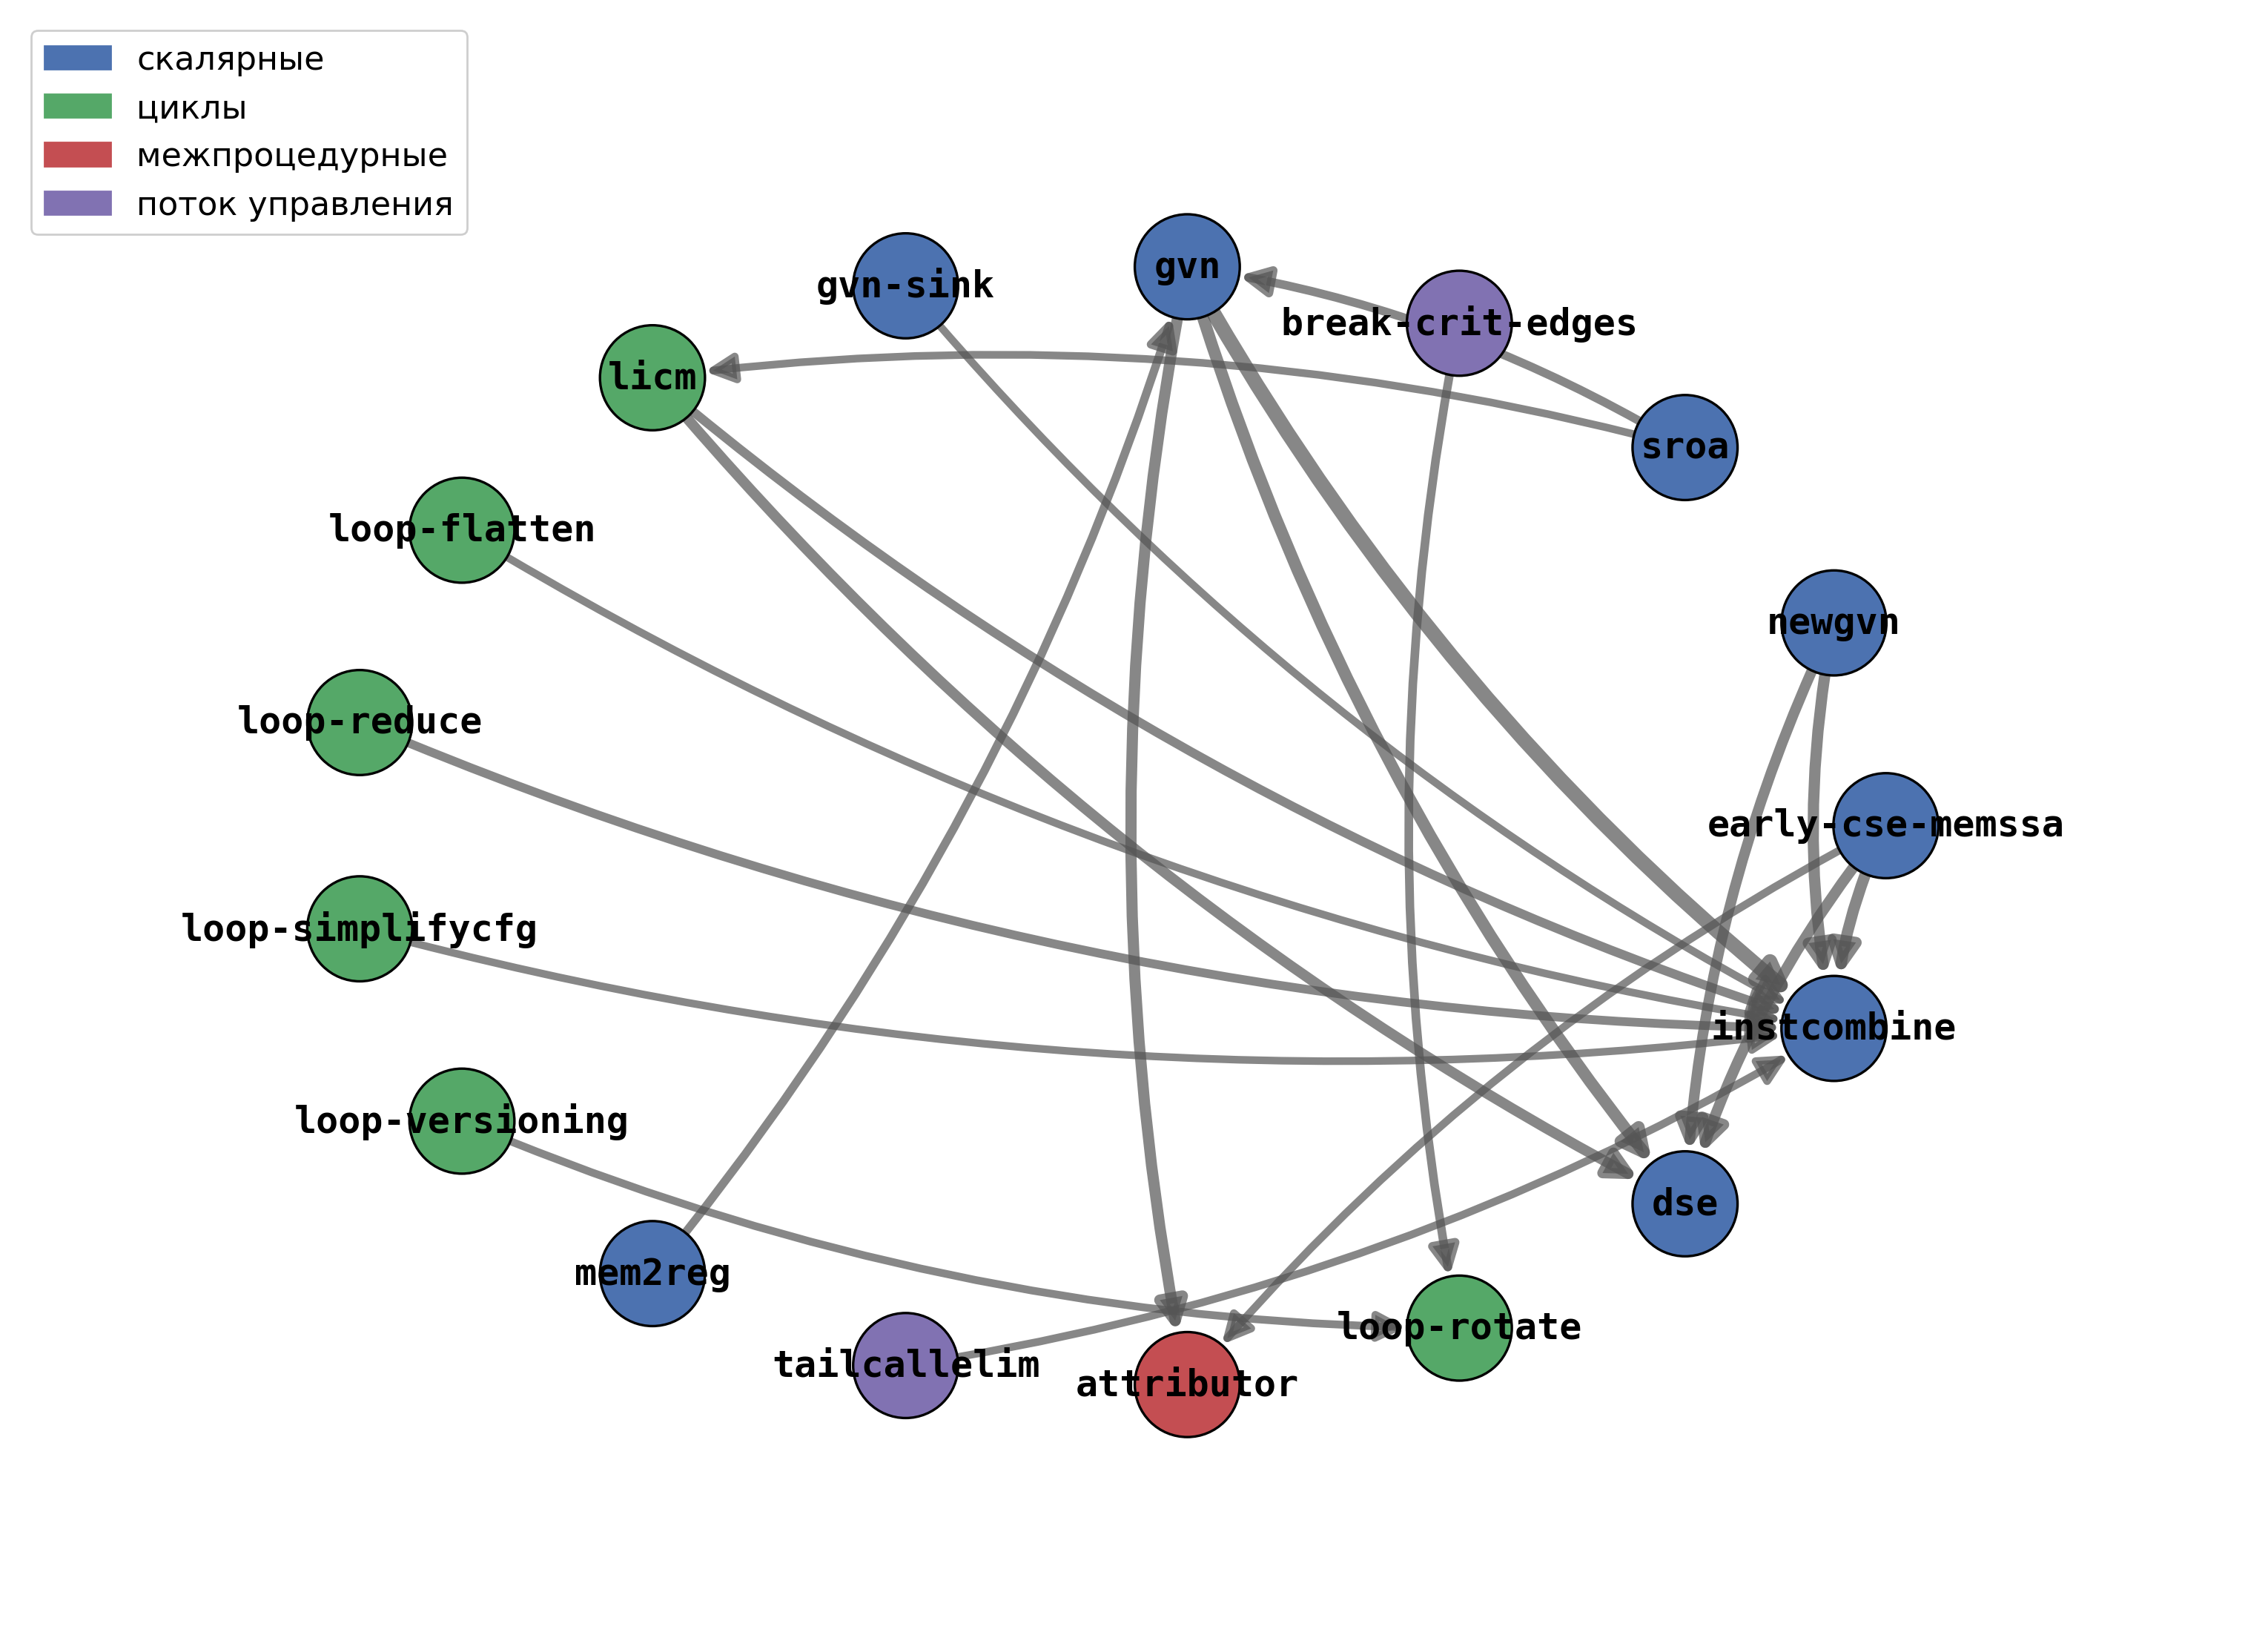
\includegraphics[width=\linewidth]{images/graph_global_top20_filtered.png}\\
      {\footnotesize Топ-20 рёбер каузального графа.}
    \end{column}
    \begin{column}{0.28\textwidth}
      \footnotesize
      Паттерн \textbf{«вычисление $\to$ упрощение»}: источники \texttt{gvn},
      \texttt{newgvn}; стоки \texttt{instcombine}, \texttt{dse}.

      \smallskip
      Рёбра \texttt{gvn}$\to$\texttt{instcombine}, \texttt{gvn}$\to$\texttt{dse}
      совпадают с \texttt{-Oz}~--- метод воспроизвёл решения LLVM.

      \smallskip
      \textbf{\texttt{-Oz} неоптимален:} лучше на \textbf{374} из 517 программ.
    \end{column}
  \end{columns}
\end{frame}

%% ================= Слайд 10: РЕЗУЛЬТАТ 2 (главный) =================
\begin{frame}{Результат 2 (главный): каузация $\ne$ корреляция}
  \centering
  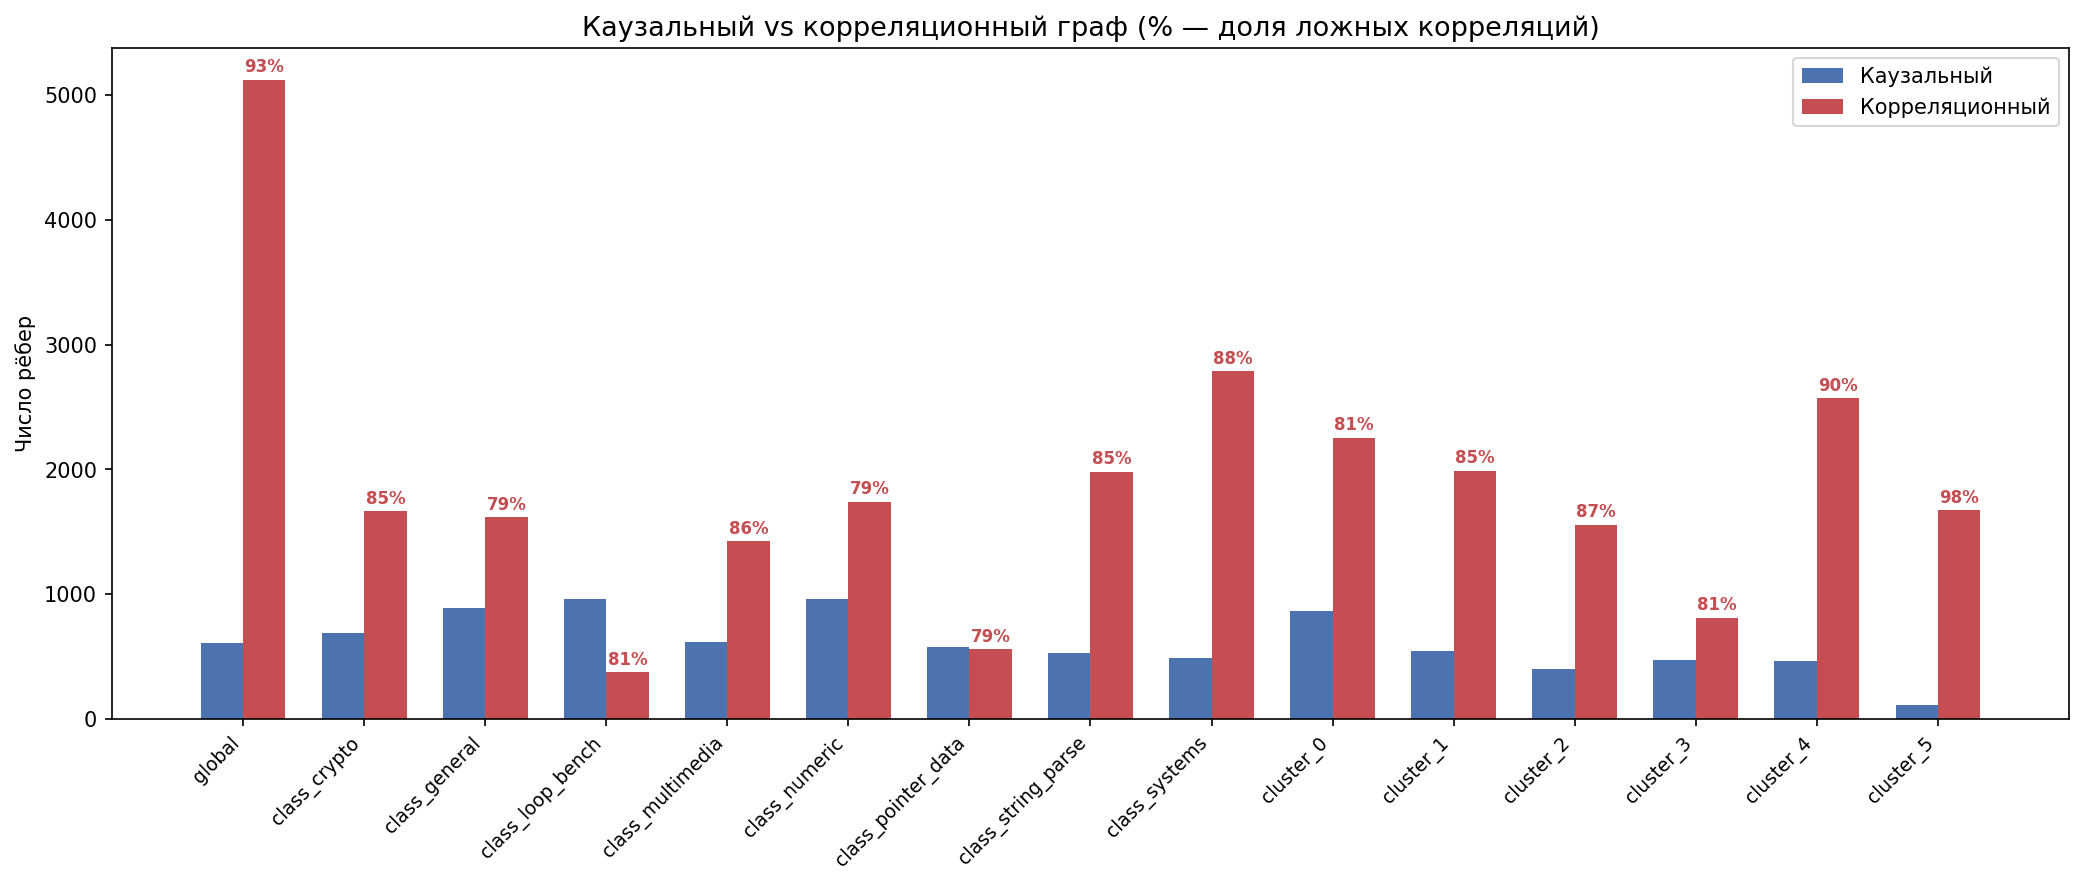
\includegraphics[width=0.88\linewidth]{images/comparison_causal_vs_corr.png}

  \smallskip
  \begin{columns}[c]
    \begin{column}{0.5\textwidth}
      \centering\small
      \begin{tabular}{@{}lr@{}}
        \toprule
        Каузальных рёбер      & \textbf{608}\\
        Корреляционных рёбер  & \textbf{5124}\\
        Пересечение           & 376\\
        \midrule
        \textbf{Доля ложных} & {\color{titlered}\textbf{92,7\,\%}}\\
        \bottomrule
      \end{tabular}
    \end{column}
    \begin{column}{0.5\textwidth}
      \small Большинство «значимых» корреляций между порядком пар и выигрышем
      \textbf{не имеют каузальной природы}~--- от 78,7\,\% (general) до 98,1\,\%
      (cluster\_5) по группам.
    \end{column}
  \end{columns}
\end{frame}

%% ================= Слайд 11: РЕЗУЛЬТАТ 3 — гетерогенность + формулировки =================
\begin{frame}{Результат 3: единого оптимального порядка нет}
  \begin{columns}[T]
    \begin{column}{0.55\textwidth}
      \centering
      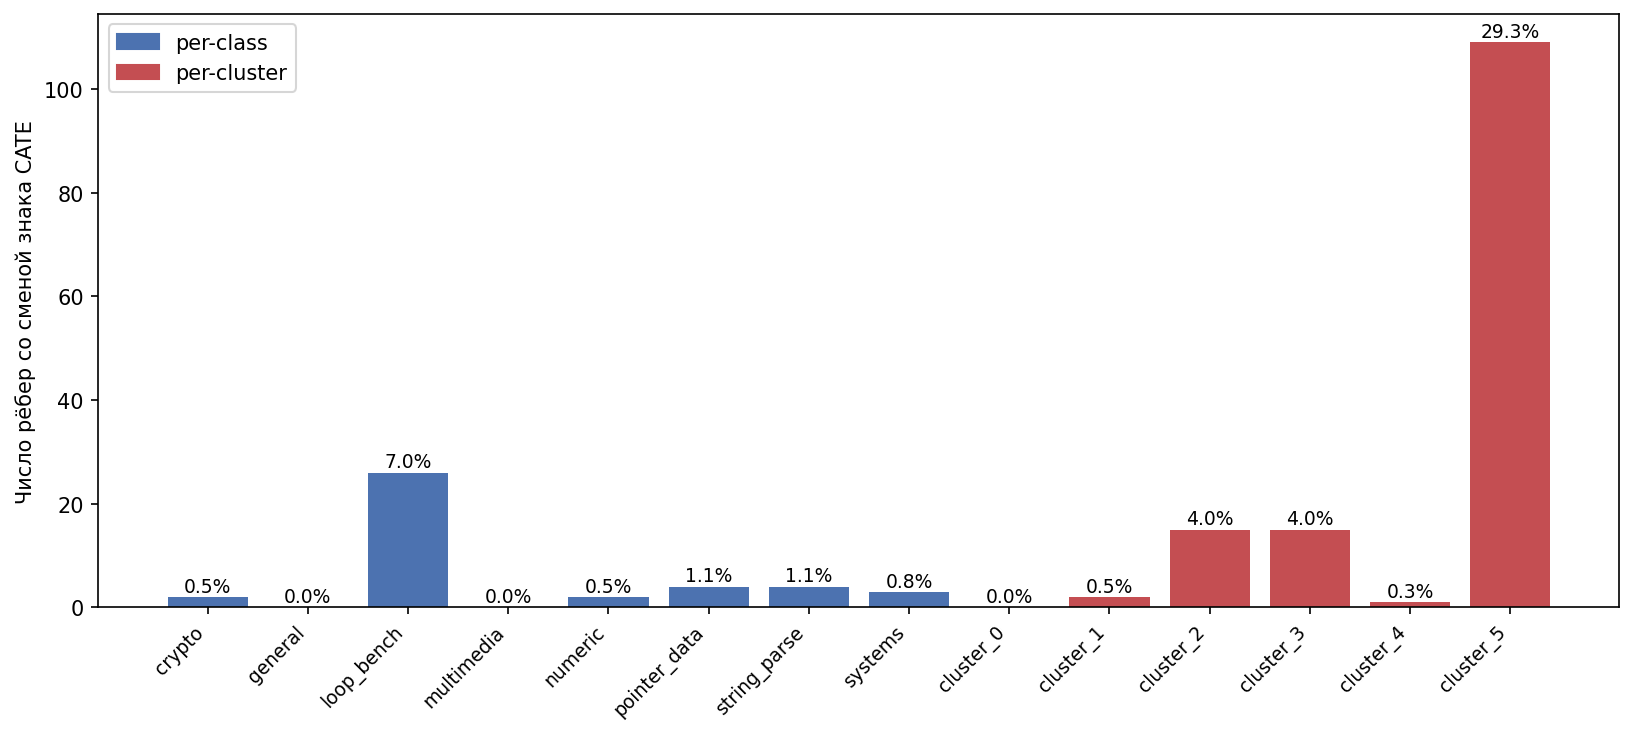
\includegraphics[width=\linewidth]{images/cate_flips_per_group.png}\\
      {\footnotesize Число рёбер, меняющих знак на подгруппе.}
    \end{column}
    \begin{column}{0.45\textwidth}
      \small
      \heading{Гетерогенность эффекта}
      Эффект порядка \textbf{зависит от типа программы}: до \textbf{29\,\%} рёбер
      глобального графа меняют знак на отдельных кластерах~--- нужны
      специализированные графы под класс программ.

      \heading{Две формулировки}
      Относительный порядок~--- \textbf{608} рёбер (глобальные зависимости),
      соседство~--- \textbf{44} ребра (локальные синергии): выявляют \textbf{разные
      классы} зависимостей.
    \end{column}
  \end{columns}
\end{frame}

%% ================= Слайд 12: ИТОГИ + положения на защиту =================
\begin{frame}{Заключение и положения, выносимые на защиту}
  \small
  Цель достигнута: построены интерпретируемые каузальные графы зависимостей
  между проходами LLVM. На защиту выносятся:
  \begin{enumerate}\setlength{\itemsep}{0pt}\setlength{\parskip}{0pt}
    \item Случайные перестановки проходов образуют рандомизированный эксперимент~---
      каузальный эффект порядка пар оценивается \textbf{напрямую}, без алгоритмов
      поиска структуры.
    \item Метод построения интерпретируемых каузальных графов на нескольких
      уровнях агрегации.
    \item \textbf{92,7\,\%} значимых корреляций «порядок--выигрыш» \textbf{ложны}
      (608 каузальных против 5124 корреляционных).
    \item Эффект порядка \textbf{гетерогенен}: до 29\,\% рёбер меняют знак по типам
      программ.
    \item Две формулировки воздействия выявляют разные зависимости (608 против 44).
  \end{enumerate}

  \smallskip
  Также самостоятельным научным вкладом является собранный датасет из
  \textbf{517} программ в LLVM IR и \textbf{5,17 млн} прогонов.
\end{frame}

%% ================= Слайд 13: публикации =================
\begin{frame}{Публикации по теме работы}
  \begin{enumerate}
    \item \emph{Белонин~В.\,В., Ефанов~Н.\,Н.} Применение методов каузального
      вывода при анализе зависимостей между оптимизирующими проходами
      LLVM-компилятора~// 68-я Всероссийская научная конференция МФТИ.~--- 2026.
  \end{enumerate}

  \vfill
  \begin{center}
    {\color{titlered}\bfseries\Large Благодарю за внимание!}
  \end{center}
  \vfill
\end{frame}

\end{document}
